\section{System Architecture}
\label{chap:hardware_architecture}
With the development of mobile payment applications comes the requirement to ensure the security of the assets involved.
Strongly related to the progression of mobile applications towards 'electronic cash' is the necessity to authenticate the transactions executed. \cite{herzberg2003payments}

%In electronic payment applications there are at least three roles to be distinguished: consumers, merchants and payment providers.
%For each inter-party transaction, the parties must be identified and authenticated.
%The problem faced by system architects in developing secure payment applications is that a breach of security can occur within each of these parties' assets.

Consumers and merchants both need to trust a payment provider to facilitate their payment transactions, and in return the payment provider must verify both parties are making rightful claims to their accounts.
There are now three participants in the transaction instead of two, and - ruling out internal sabotage - two points of potential malice rather than just one.
This creates a situation where the burden to authenticate a transaction is twice as great on the payment provider as it would be for either participant in a direct two-party transaction.

Traditional mechanisms of authenticating the card holder rely on verification of the signature and visual inspection of the card.
Verifying transactions more efficiently can be achieved using a cryptographic solution, where the user and payment provider are in possession of a \textit{shared secret}.
%A more secure means of verifying transactions would be a mechanism where the user would.
The payment provider would share with the user two secrets: one which is known only to the payment provider while in possession of the user, whereas the other secret is known to both parties.
This secret unknown to the user can be thought of as a padlock which the user can close, but not open.
It may be in the user's possession, but extracting the combination from the lock would in most cases destroy it.
Using this lock, the user can transmit the 'locked' shared secret to the payment provider in order to authenticate his or her transaction.

%A technical solution to the authentication problem could be achieved using cryptography.

%A payment provider
%TODO Leg uit hoe je met trust omgaat in electronisch bankieren

\textit{Integrated Circuit Cards} (ICCs), commonly known as smartcards or chip cards, are cards which contain an integrated circuit system that communicate via contact points on the chip.
ICCs can be used to cryptographically sign data using a preconfigured secret key known only to the issuer of the card.
%By design, there is no way to retrieve the secret key from the device, accomplished 
ICCs can be issued with various anti-tampering mechanisms, adding to the intrinsic tamper-resistance of the embedded microchip itself due to its small scale. \cite{kömmerling1999design}
Europay, Mastercard and Visa have jointly designed the EMV standard for smart card interoperability describing a secure means of transaction authentication. %, which has been largely adopted by the banking industry and is in widespread use.
Smart cards used in EMV hold a cypher and secret key known only to the bank, which are used to sign transactions.
%This standard has been adopted by the banking industry which has lead to the widespread deployment of smart cards in banking.
%Smart cards are called 'smart' because they contain an embedded microchip which is able to not only store data, but also run code.

Modern RFID cards can have features similar to smart cards, which means that NFC devices aiming to be truly backward compatible with RFID applications must also allow for similar functionality.
This requires a secure storage and processing module to be included in the design of NFC devices as conventional storage on and operation of mobile devices are liable to tampering by the user.
%NFC, being grounded in RFID technology, provides some security capabilities previously unavailable in mobile devices.
%These capabilities require storage of sensitive data and code, for which a \textit{Secure element} is needed.

Most mobile telephones make use of the \textit{Global System for Mobile Communications} (GSM) system.
The GSM standard already provides a mechanism for identification and authentication on the network by means of a smart card, albeit in a different form factor.
These are called \textit{Universal Integrated Circuit Cards} (UICCs).
Besides storing the secret key, the card is running a \textit{Subscriber Identify Module} (SIM) application, which holds the routines used for encryption in GSM, so that the secret key never needs to leave the SIM card. % TODO referentie

\begin{figure}
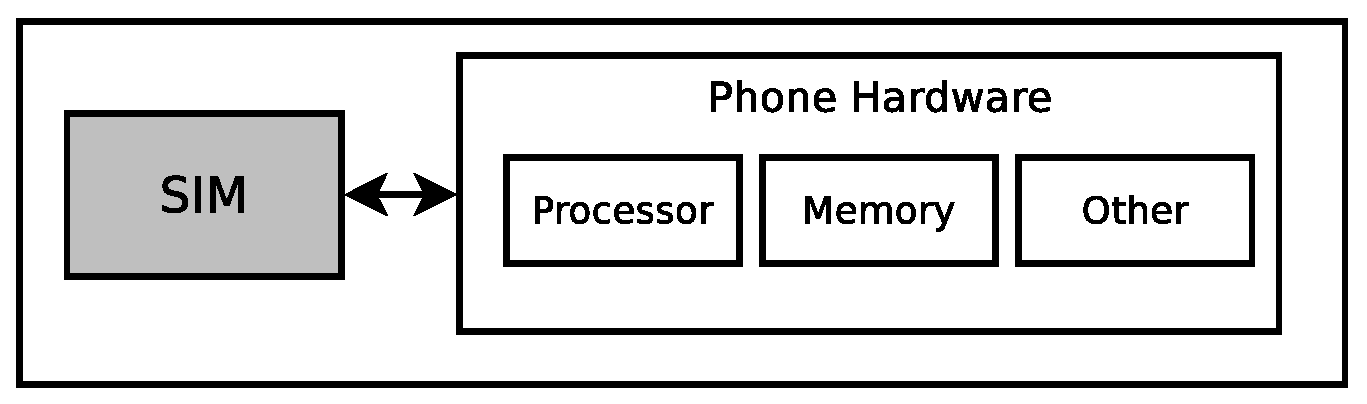
\includegraphics[width=0.9\textwidth]{images/SIM_in_GSM}
\caption[UICC running SIM application in GSM]
{
A UICC (SIM) card as used in GSM.
}
\label{fig:gsm_sim}
\end{figure}

In fact these cards, also known as SIM cards, remain property of the telco after distribution, much like a bank card or passport remain the property of their respective issuers. %TODO referentie
Due to this, the current generation of mobile devices lack a common infrastructure for third parties to make use of such secure storage for their own applications.

%These third parties need to be elevated to the role of \textit{Trusted Service Manger}
%MARK: In de tekst hieronder moet duidelijk worden, dat NFC eist/vraagt dat een UICC wordt opgedeeld voor verschillende applicaties

% ERIK: SIM is een voorbeeld van een "Secure Element". Een Secure Element kan ook een andere smartcard chip in de telefoon zijn.

% In de telefoons die 'we' hebben is de SE geen onderdeel van de SIM, maar een los (al dan niet trusted) component.
%MARK: zullen we dit verder uitbreiden in het architectuur hoofdstuk en dit hier niet noemen?


%ERIK Waarom is de architectuur van GSM zoals-ie is & hoe breidt NFC dat uit? Er zijn tig opties van NFC telefoons, dus we kunnen niet overal diep op ingaan.

%TODO afmaken :)
\subsection{Secure elements}
%TODO citation geen onderwerp maken
%Currently, four different configurations for a secure element are possible, of which the integration on a regular UICC/SIM is suggested as the most likely candidate to be used.
Secure Elements can be implemented in mobile devices to facilitate the secure storage / execution.
Several possible configurations proposed by \textit{GlobalPlatform}, the industry forum for smart card infrastructure development, are outlined below. \cite{Reveilhac:2009:PSE:1548884.1549404,GlobalPlatformSEs}
%The secure element to be used is a \textit{Universal Integrated Circuit Card} (UICC).
%This is a smartcard which is used in a mobile phone to connect to the GSM and UTMS network. % UICC toevoegen aan glossary, Uitleggen dat het SIM is
%Making use of a UICC is preferred because it has been deployed in real applications where it has proven to be reliable.
%It is re-usable and standardized, which means a user can switch handsets easily, their personalized secure. 


%\textbf{TODO}
%A good reference on the feasibility of secure data and code in mobile devices is given in \cite{Reveilhac:2009:PSE:1548884.1549404}.
%Explain that the technical workings of these different devices are equivalent, but different configurations belong in different trust models.


%ERIK: figuren toevoegen van verschillende telefoon architecturen. 

% SIM ---> telefoon		SIM = secure, tamper-resitent, authenticatie van telefoon aan het netwerk	marketing redenen (onderscheid welke onderdelen van wie zijn) SIM is van de telco
% a SIM ---> telefoon ---> SE 	SmartMX contactless smartcard  (nokia)
% b SD kaart als a maar vervangbaar SE
% c NFC-SIM

%The problem of a malicious user can be mitigated by making use of a \textit{Secure Element} (SE) for storing sensitive information.
%Because of its sheer microscopic scale, it is very difficult and costly for an attacker to tamper with the function of this device.

%Below we will discuss a number of different ways such a secure element can be implemented on a mobile device. 

%\subsubsection{Integrated Secure Element}
One option would be to integrate the SE in the handset hardware directly.
This works for the intended cryptographic use, but limits the device to communicate with the services aware of its pre-programmed secret key, unless it is capable of securely updating itself with news keys.

Nokia has released a phone like this in 2006 (the Nokia 6131 NFC) . %with NFC as a feature.
The architecture of this phone consists of a SIM card, antenna and an internal Secure Element.
The same layout of this architecture can also be used in other mobile devices, see figure \ref{fig:integrated_se}.

The phone hardware consists of the usual (processor, memory), but also hardware to provide for NFC features and a secure element to enable payment and ticketing.
The secure element stores sensitive data and enables tag and smart card emulation.
In the case of the Nokia phone it is divided in two subcomponents, a Java Card, used for payment, and Mifare 4k, used for ticketing.

\begin{figure}
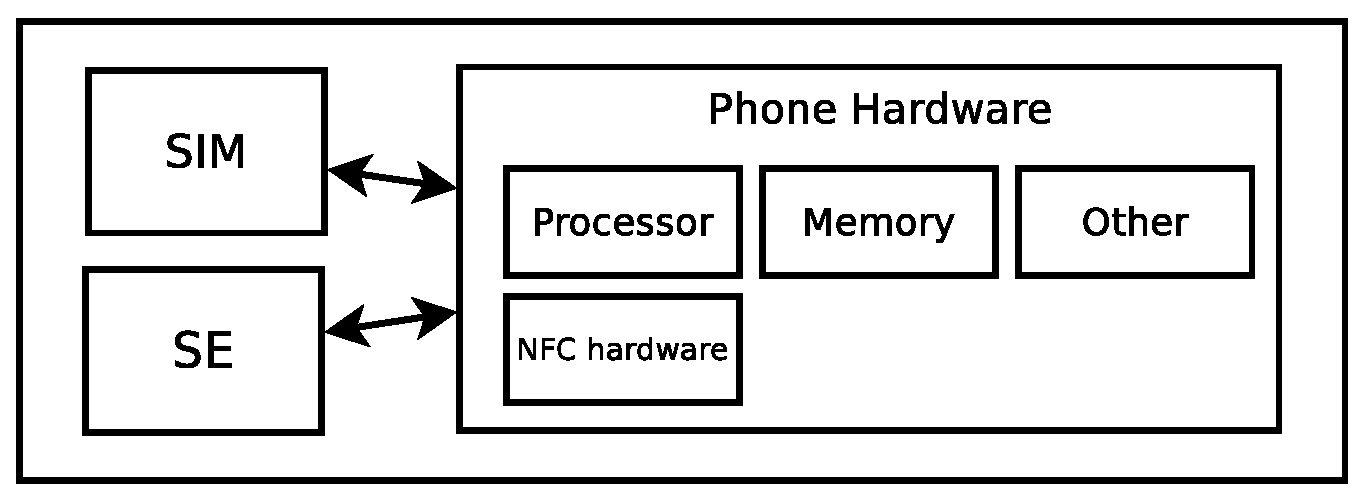
\includegraphics[width=0.9\textwidth]{images/phone_with_SE_nokia}
\caption[Nokia phone with SE]
{
A separate secure element
}
\label{fig:integrated_se}
\end{figure}


%security problems for this architecture:

%\subsubsection{Modular Secure Element}
Another option is an external SD-card which houses all the hardware needed to enable NFC and also the secure element, see figure \ref{fig:modular_se}.
%( http://www.nearfieldcommunicationsworld.com/2009/01/12/3485/tyfone-puts-nfc-into-microsd-cards/)
In this configuration a third party can issue an SD card to its customers which houses a secret key hidden from the user.

\begin{figure}
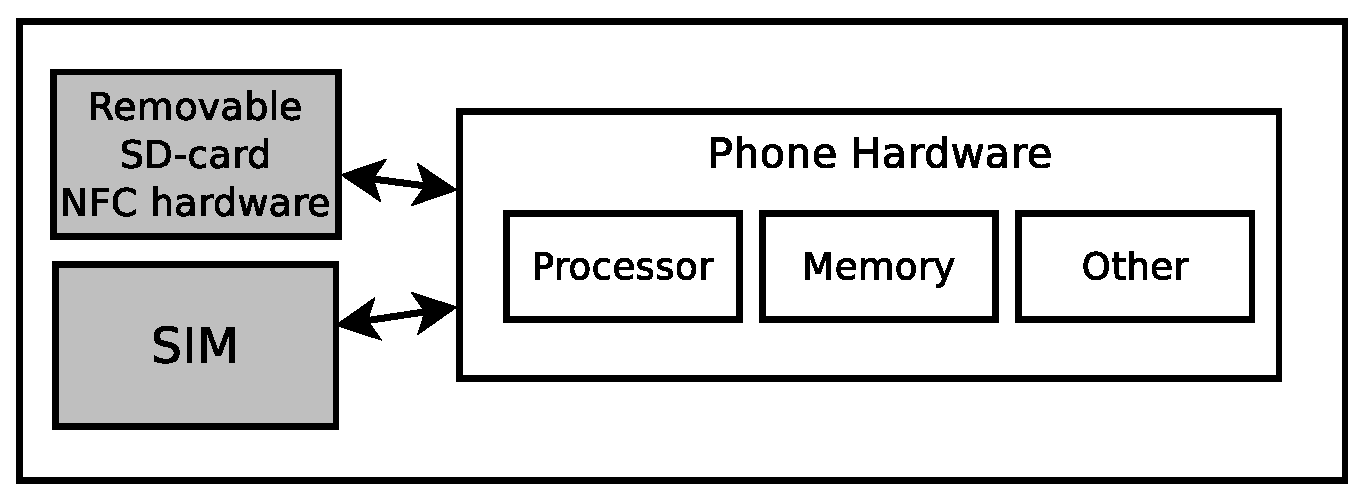
\includegraphics[width=0.9\textwidth]{images/SD_NFC}
\caption[SE in SD package]
{
An secure element in SD package
}
\label{fig:modular_se}
\end{figure}

%security problems for this architecture: SD card might get stolen and used by somebody else.
%\subsubsection{Multiple SIM cards}
Related to the above architecture is the one depicted in figure \ref{fig:multi_sim}.
Here the architecture consist of a phone with multiple SIM cards and the usual hardware.
In this case a telecom provider will own one SIM card and third-party service provider will own the other.
This way there no problem with splitting the resources of one SIM card and the trust issue between different companies.
\begin{figure}
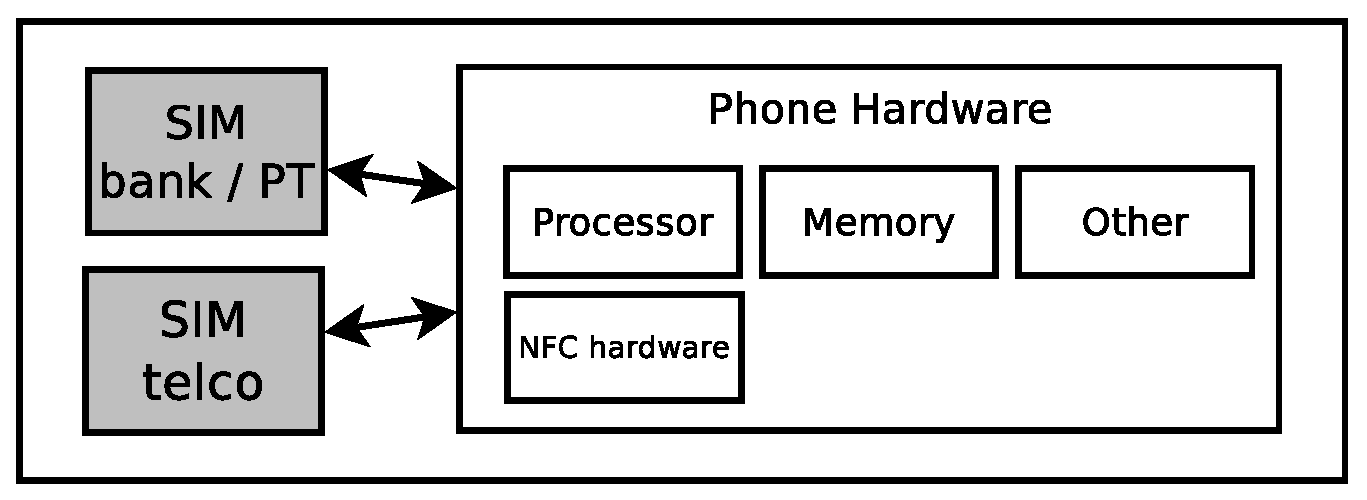
\includegraphics[width=0.9\textwidth]{images/meerdere_sims}
\caption[Multiple SIM cards]
{
Multiple SIM cards for different applications
}
\label{fig:multi_sim}
\end{figure}

%\subsubsection{Trusted SIM card}
Of course the option of splitting the resources is also possible, if different companies can find an agreement to share the same SIM card.
This is possible, because smartcards in general are becoming more powerful.
This makes two different architectures possible.
The first one, as pictured in figure \ref{fig:sim_se}, uses the SIM card as secure element.
A phone will have the usual hardware, hardware making NFC possible and SIM card with applications from the telecom provider and applications from a company chosen by the user, e.g. a bank for payment and a public transport company. 
The second option resembles a combination of the first one and the one with the SD card architecture.
Here a SIM card has all the hardware needed to make NFC possible and it also acts as a secure element (see figure \ref{fig:integrated_se}).
Like the first option, the resources of the SIM card will be split among the involved parties.
\begin{figure}
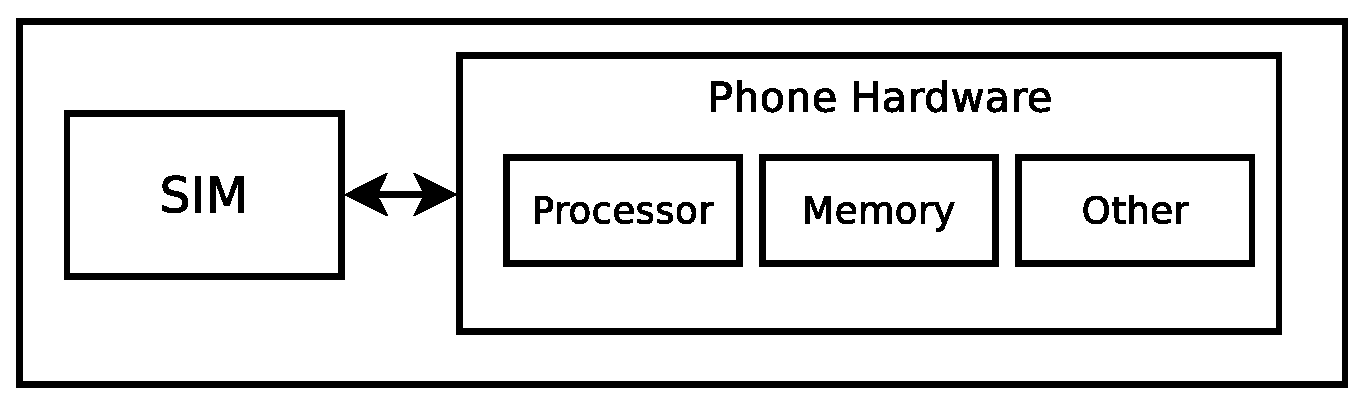
\includegraphics[width=0.9\textwidth]{images/SIM_is_SE}
\caption[Trusted SIM cards]
{
Trusted SIM card running multiple applications
}
\label{fig:sim_se}
\end{figure}

%hier moet nog een bron voor gevonden worden
%security problems for this architecture: SIM card might get stolen and used by somebody else
%hier moet nog een bron voor gevonden worden
%security problems for this architecture: SIM card might get stolen and used by somebody else


\subsection{Adoption of NFC}
In \cite{1497411} the authors investigate the possibility of running trusted code in mobile devices and concluded that while such a system is technically feasible, its widespread adoption is hampered by the certification process payment card companies impose on their payment products.
Payment card companies' current standards dictate that their cards may not be modified after production, which poses a problem as this is exactly what makes NFC an enticing alternative to conventional bank cards.

This poses a problem for the implemention of NFC in general.
As seen in (figure xx, still to add) the "demand" for NFC is a circular dependency.
If the customer doesn't demand NFC from an issuer (bank, PT), the issuer won't request a TSM to create application, so nothing will be putt on a UICC by the MNO and the customer gets nothing.
If one of the parties in this figure, refuses to cooperate, NFC will not launch.
What we see now (artikel tweakers en global platform) is that issuers and MNO are working together to make NFC available for customers.
The next thing to happen is that mobile phones will get NFC hardware and an implementation of a secure element.
With Nokia's 6131 NFC phone a first step was made for developers.
But now also Google has announced that they will introduce a NFC phone and some rumours suggest that also Apple is developing a new Iphone with NFC, see \cite{nu_artikel}.
If customers like NFC because of the possibilities it will take off and demands for other applications will be made. 

\textbf{TODO} A good reference for cyclic dependency of stakeholders can be found in the GlobalPlatform technical report.


% TODO hoort bij Wireless communication, terwijl 3.2 (Secure Elements) heel ergens anders over gaat
%\subsection{Standardization}
%NFC has been described by NFCIP-1 (Near Field Communication Interface Protocol 1) first on ISO18092, ECMA340 and ETSI %TS102 and also NFCIP-2 defined in ISO 21481, ECMA352 and ETSI TS102 312.
%With NFCIP-2, NFC became compliant with the RFID standards of ISO14443 and ISO15693.


% diagram van NFC communicatie

%TODO RFiD card vs NFC - verschil vd terminal
%                      - live GSM verbinding met de bank
%TODO Online vs Offline
%                      - privacy gevoeligheid

%\section{Wireless communication}
%The distance at which the NFC communication takes place is 10 cm, operates at the 13.56 MHz frequency and it has a transfer speed of 106, 216, 424 kbit/s.
%promising secure element alternatives for NFC technology. */


%\subsection{Advantages and Limitations}
%\textbf{TODO}

% Toetsenbord en display feature (semi-trusted terminal, moeilijker te tamperen)

% Voorbeeld telefoon met gewone sim en NFC SD card adapter
% Bankier kan heir apps op installeren

% Voorbeeld telefoon met meerdere sims

% Vorobeeld SIM en losse SE, met trusted code

% Voorbeeld SIM van KPN, met apps van de bank

%TODO Uitzoeken:
% Rabomobiel - SIM vd rabobank


